%%%%%%%%%%%%%%%%%%%%%%%%%%%%%%%%%%%%%%%%%%%%%%%%%%%%%%%%%%%%%%%%%%%%%%%%%%%
%% This file is part of the book
%%
%% Algorithmic Graph Theory
%% http://code.google.com/p/graph-theory-algorithms-book/
%%
%% Copyright (C) 2009--2011 Minh Van Nguyen <nguyenminh2@gmail.com>
%%
%% See the file COPYING for copying conditions.
%%%%%%%%%%%%%%%%%%%%%%%%%%%%%%%%%%%%%%%%%%%%%%%%%%%%%%%%%%%%%%%%%%%%%%%%%%%

\documentclass{article}

\usepackage{tikz}
\usetikzlibrary{external}
\tikzexternalize{tree-representation-B-2}

\begin{document}

\begin{figure}
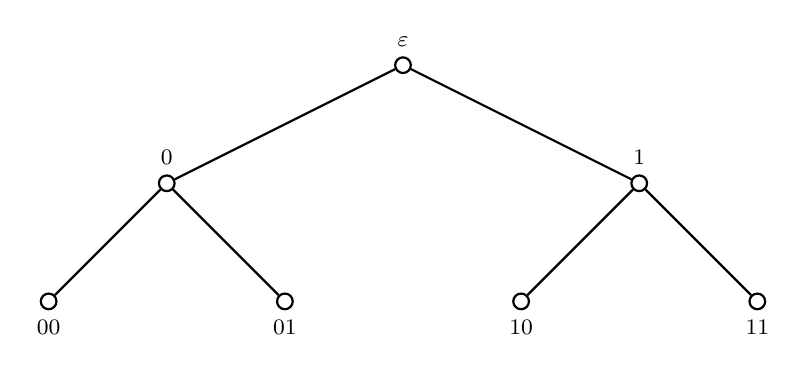
\begin{tikzpicture}
[lineDecorate/.style={-,thick},%
  nodeDecorate/.style={shape=circle,inner sep=2pt,draw,thick},%
  scale=1.5]
%% nodes or vertices
\foreach \nodename/\x/\y/\direction/\navigate in {
  00/0/0/below/south, 01/2/0/below/south, 10/4/0/below/south,
  11/6/0/below/south, 0/1/1/above/north, 1/5/1/above/north}
{
  \node (\nodename) at (\x,\y) [nodeDecorate] {};
  \node [\direction] at (\nodename.\navigate) {\footnotesize$\nodename$};
}
\node (e) at (3,2) [nodeDecorate] {};
\node [above] at (e.north) {\footnotesize$\varepsilon$};
%% edges or lines
\path
\foreach \startnode/\endnode in {0/00, 0/01, 1/10, 1/11, e/0, e/1}
{
  (\startnode) edge[lineDecorate] node {} (\endnode)
};
\end{tikzpicture}
\end{figure}

\end{document}
